\section{Robust Extraction}
\label{section:extraction}
The PTA algorithm enables us to generate a fixed rule (XPath) to extract data from the given pages.
However, XPath is heavily reliant on the structure of the DOM page in its present form: Any element
extracted is defined by its ancestor nodes and their attributes. Once this is changed, which is
likely due to a layout change, the same XPath may no longer be applicable to the current page. 

In order to be able to extract data even after a change in layout, another method of extraction
without the use of XPath is required. Our approach for this system uses a machine learned model.
The rest of the chapter elaborates on the details of the implementation.

In our framework, we use the provided XPaths together with the URLs of the pages to be extracted
as annotated documents. Each node in the DOM is treated as a separate instance, and labelled
based on the XPath it was extracted by. The XPaths are assumed to be mutually exclusive. We have
chosen to use decision trees because the generated models are small, and can be easily interpreted.
The generation of these models are also relatively faster than other classification models. Since
CPU time and memory space are constrained resources, decision trees were suitable for our needs.

	
Looking at any web information extraction system using machine learning classification techniques, the workflow of a user can be generalised into the following steps:
\begin{enumerate}
	\item The user finds a page or site that he/she would like information to be mined from.
	\item Samples of the page presented to the user for labelling. Positive examples are selected and these are fed into the machine learner to create a model.
	\item Using this model, data is extracted from similar pages, this data is then put into storage (e.g. database)
	\item Some systems repeat steps 2 and 3 iteratively until an accurate model is achieved. \label{repeatstep}
	\item The user can then access the data storage for the mined information.
\end{enumerate}

Our system follows the same workflow, except for step \ref{repeatstep}. We will elaborate further
how the machine learning component fits into the entire picture in \ref{chap:implementation}.

\subsection{Features used}
To keep the model more robust and resistant to layout changes on the original site, content features are extracted in order to use less of the HTML structure for extraction. In this system, a J48 decision tree classifier is used. Positive examples of HTML elements are those returned when the XPath is applied to the given page. The following features are extracted:

	\begin{itemize}
		\item Word occurrence count, or tokens (Numeric)
		\item Tag name (Discrete)
		\item Previous sibling, next sibling and parent tag name (Discrete)
		\item Number of words/tokens (Numeric)
		\item Ending with character (:,-,.) (Discrete)
		\item Header (Discrete)
	\end{itemize}
	

	
	%need to run more tests on SVMs and dec trees
	
	For subsequent extractions, the server will first use the available XPath for extraction from the site.
	If the XPath rule fails to find elements for extraction, the learnt classification model is used. Figure
	\ref{fig:decisiontree} shows a decision tree when the process is run on a Google search result with the
	result entries selected for extraction.

\begin{figure}[htbp]
\centering
% Set the overall layout of the tree
\tikzstyle{level 1}=[level distance=4cm, sibling distance=3.5cm]
\tikzstyle{level 2}=[level distance=4cm, sibling distance=2cm]

% Define styles for bags and leafs
\tikzstyle{bag} = [text width=4em, text centered]
\tikzstyle{end} = [circle, minimum width=3pt,fill, inner sep=0pt]
\tikzstyle{fork} = [circle, minimum width=3pt,fill, inner sep=0pt]
% The sloped option gives rotated edge labels. Personally
% I find sloped labels a bit difficult to read. Remove the sloped options
% to get horizontal labels. 
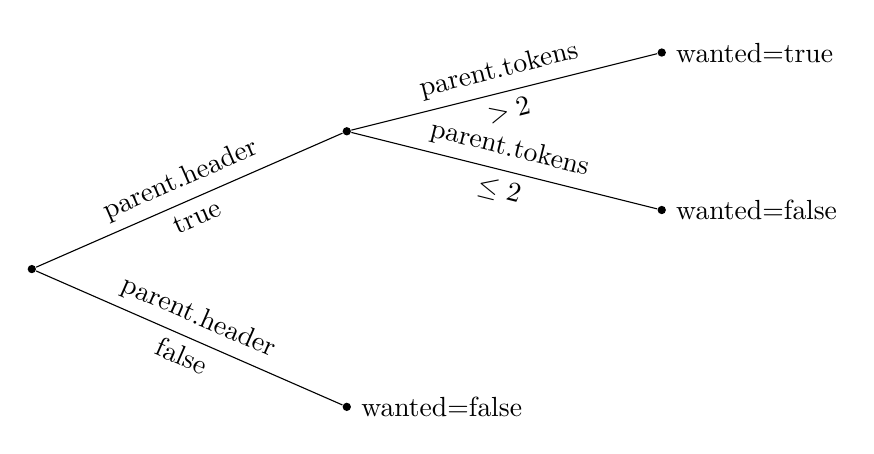
\begin{tikzpicture}[grow=right, sloped]
\node[fork] {}
    child {
        node[end, label=right:
                    {\url{wanted=false}}]{}      
	edge from parent 
            node[above] {\url{parent.header}}
            node[below]  {\url{false}}
    }
    child {
        node[fork]{}   
        child {
                node[end, label=right:
                    {\url{wanted=false}}] {}
                edge from parent
                node[above] {\url{parent.tokens}}
                node[below]  {$\leq 2$}
            }
            child {
                node[end, label=right:
                    {\url{wanted=true}}] {}
                edge from parent
                node[above] {\url{parent.tokens}}
                node[below]  {$>2$}
            }
        edge from parent         
            node[above] {\url{parent.header}}
            node[below]  {\url{true}}
    };
\end{tikzpicture}
\caption{Decision tree generated when search entries on Google are selected.}
\label{fig:decisiontree}
\end{figure}
	
	As we can see, the generated decision tree seems pretty reasonable given a Google search result. The
	\url{parent.}	prefix is the equivalent to the statement ``if the parent of the element". We can see
	that the generated tree is looking for elements with parents that are headers and contain 2 or more words.
	
\subsection{Crawling for more instances}
	We found that many annotations capture very few elements per page when compared to the total number of elements for that page. By attempting to balance the number of elements that belong to labels with those that were not captured by any XPath, we hoped to improve the performance of the classifier. However, this still yielded relatively poor results. Eventually, we crawled the site for other pages which had elements captured by the same set of XPaths. This gave us more instances to train the classifier on, and gave better results.
	
The crawler starts with a given set of pages, and crawls links with URLs similar to the given pages. The similarity score is given by the edit distance between the link URL and the URL of the wanted pages. A heap is used to store the seen links, and the most similar URL selected at every round. The crawler stops when it has collected a fixed number of instances, which is now set at 500.
	
\subsection{Limitations}
In Weka's implementation of their machine learning algorithms, the serialised models created
tend to store all attributes and their values. Due to this, some of the models are really large,
with a lot of redundant data. This takes up much I/O time and storage space on the server. However,
in comparison with the implementations of the other classification methods in the Weka 
library, the decision tree classifier does perform better than the other classifiers in terms
of runtime and model size. A decision tree classifier optimised specifically for the system
was not implemented due to time constraints.

Also, from our tests, the learnt model does better on heading-type results, while other
fields tend to have a low precision score, we will discuss the evaluation results in detail
in Chapter 4.
	
	

